%======================================================================
\chapter{Background}
%======================================================================
\section{Natural Language Processing}
Natural Language Processing is the branch of artificial intelligence that deals with providing computers with the ability to understand text and spoken words, similar to how human being do \cite{Khurana:2023}. \gls{NLP} includes tasks such as summarization, sentiment analysis, and spam detection \cite{Khurana:2023}.

One significant advancement within \gls{NLP} was the introduction of \gls{transformer} models \cite{Vaswani:2017}. Before the introduction of Transformers within NLP, neural networks such as word2vec \cite{Mikolov:2013} and GloVe \cite{Pennington:2014} generated contextual independent embedding vectors for words. Transformer models such as T5, BERT, ALBERT, RoBERTa, and XLNet outperformed these models with the introduction of contextual embeddings generated through self-attention \cite{Vaswani:2017}.

The \gls{transformer} models used in \gls{NLP} vary significantly. Examples of differences between models includes with architecture, training procedure, and size. These differences contribute to different use cases and performance between models. The models used in the \textit{E}-score method for protein sequence alignment are based on the models introduced below for NLP. Comparison between the GLUE benchmark scores for these models is shown in Table \ref{tab:glue}

\subsection{T5}
\gls{T5} uses a text-to-text approach using the \gls{transformer} architecture. That is, T5's input and output are always text strings \cite{Raffel:2020}. It uses both the encoder and decoder from the transformer architecture, and relies on \gls{transfer learning} to fine-tune the model on downstream tasks. An example of T5's input and output is shown in Figure \ref{fig:t5example}.

\begin{figure}
    \begin{center}
	   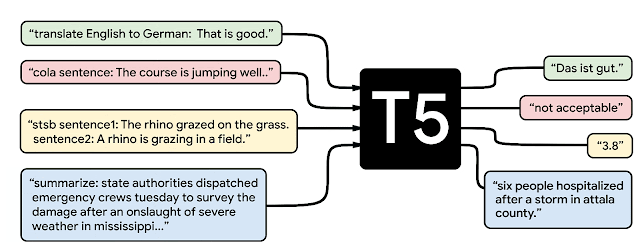
\includegraphics[width=0.75\linewidth]{figures/t5example.png}
    \end{center}
    \caption{Diagram of T5's text-to-text framework. Each task uses text as the model input, which is trained to generate some target text \cite{Raffel:2020}.}
    \label{fig:t5example}
\end{figure}

By training \gls{T5} with fill-in-the-blank-style \gls{denoising} objectives, where T5 was trained to recover missing words in the input, and using transfer learning on smaller labeled datasets, T5 was able to achieve state-of-the-art \gls{NLP} performance \cite{Raffel:2020}.

\subsection{BERT, ALBERT, and RoBERTa}
\gls{BERT} achieved state-of-the-art \gls{NLP} performance at the time of it being published \cite{Devlin:2018}. ALBERT and RoBERTa are both derivations of BERT, and \gls{T5} also drew significant inspiration from BERT, such as the \gls{denoising} objective being inspired by BERT's masked language modeling objective.

\gls{BERT} is an encoder-only model that applies bidirectional training using the "masked language modeling" objective that was created for the model. This contrasts the previous framework where models read the text input sequentially, allowing for a deeper sense of context. Masked Language Modeling works by replacing 15\% of the words in an input sequence being replaced with a "MASK" token, which the model attempts to predict the original value of based on the context from the other words \cite{Devlin:2018}.

\gls{ALBERT} addresses the limitations of training time and GPU/TPU memory by presenting parameter-reduction techniques for \gls{BERT} \cite{Zhenzhong:2020}.

\gls{RoBERTa} addresses the observation that \gls{BERT} was significantly under-trained. RoBERTa improved upon BERT by training longer, removing the next-sentence pretraining objective from BERT, and training with larger mini-batches and learning rates \cite{Liu:2019}.

\subsection{XLNet}
XLNet is a model that overcomes the pretrain-finetune discrepency that \gls{BERT} suffers from because it relies on masking the input during training \cite{Yang:2022}. XLNet is a decoder-only model (also known as autoregressive) that overcomes BERT's limitations because of it's autoregressive formulation.

XLNet outperforms \gls{BERT} significantly on 20 tasks, such as question answering and sentiment analysis \cite{Yang:2022}.

\begin{table*} % Two column table
	\caption{GLUE benchmark scores \cite{Wang:2019} for the Natural Language Processing models that serve as foundation for the \textit{E}-score models.}
	\centering
    \vspace{1mm}
	\begin{tabular}{ |c|c|c|c|c|c|c|c|c|c|c| }
		\toprule
		Model & Avg & CoLA & SST-2 & MRPC & STS-B & QQP & MNLI & RTE & WNLI\\
		\midrule
		T5 & 88.7 & 71.6 & 97.5 & 92.8 & 93.1 & 75.1 & 92.1 & 92.8 & 94.5 \\
        XLNet & 87.5 & 70.2 & 97.1 & 92.9 & 93.0 & 74.7 & 90.9 & 88.5 & 92.5\\
		ALBERT & 87.3 & 69.1 & 97.1 & 93.4 & 92.5 & 74.2 & 91.1 & 89.2 & 91.8\\
        RoBERTa & 86.4 & 67.8 & 96.7 & 92.3 & 92.2 & 74.3 & 90.5 & 88.2 & 89.0 \\
		\bottomrule
	\end{tabular}
	\label{tab:glue}
\end{table*}

\section{Sequence alignment}
Sequence similarity is essential in sequence analysis within bioinformatics \cite{Ofer:2021}. Peptide sequence alignment is the most complex case, with a language of 20 common \gls{amino acids} forming a theoretically countably infinite amount of unique \gls{peptide} sequences shown in Equation \ref{eq:peptideinfinity} by taking the n-ary Cartesian product.

\begin{equation}
    {Theoretical\, Limit} = \prod_{k=1}^{\infty} |A| = \prod_{k=1}^{\infty} 20 = 20 \times 20 \times \ldots
    \label{eq:peptideinfinity}
\end{equation}

While there is theoretically a countably infinite number of \gls{peptide} sequences, the observed sequences in living organisms are constrained by biological, genetic, and functional factors. For example, the average eukaryotic protein size is \(353 \pm 62.5\) \glspl{residue} \cite{Nevers:2023}. 

Databases such as UniProt \cite{UniProt:2023} and PeptideAtlas \cite{PeptideAtlas:2006} are repositories filled with \gls{peptide} sequences. UniProt contains over 250 million unique peptide sequences and counting, showcased in Figure \ref{fig:uniprot}.

\begin{figure}
    \begin{center}
	   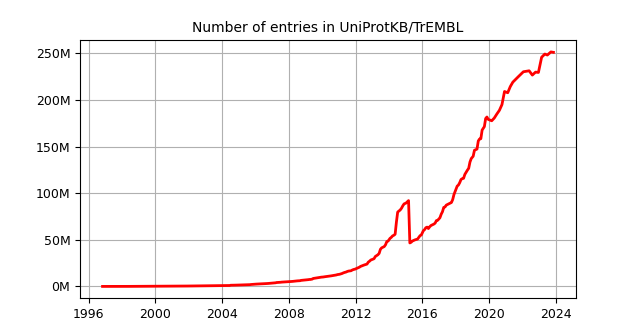
\includegraphics[width=0.75\linewidth]{figures/uniprot.png}
    \end{center}
    \caption{UniProtKB protein database release statistics as of May 2023 \cite{UniProt:2023}.}
    \label{fig:uniprot}
\end{figure}

Peptide sequences are not completely random because of the constraints imposed on them. Similar to letters or words in a given language within natural language, the frequency of each amino acid observed in nature is not equally distributed \cite{Beals:1999}, which can be observed in Figure \ref{fig:aafreq}.

\begin{figure}
    \begin{center}
	   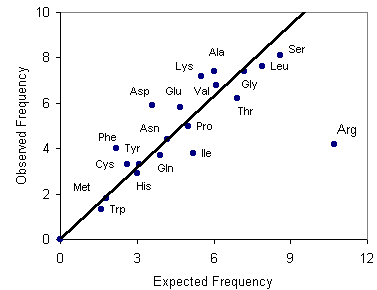
\includegraphics[width=0.5\linewidth]{figures/aafreq.png}
    \end{center}
    \caption{Observed frequency versus expected frequency of the 20 amino acids in vertebrates \cite{Beals:1999}}
    \label{fig:aafreq}
\end{figure}

Proteins are also not completely random and form different secondary structures as part of the tertiary and quaternary structure of a protein. The most common of these secondary structures are \(\alpha\) helices and \(\beta\) pleated sheets \cite{Ma:2018}. Because of the nature of proteins, algorithms such as an \gls{ENNA} are able to distinguish natural proteins from randomly generated proteins with an accuracy of over 94\% \cite{Lucrezia:2012}.

Finding similarities among protein sequences is essential in identifying protein structure and function. This is done by computing alignments between sequences. The \gls{BLAST} program\footnote{Exceeds 108,000 citations, according to Google Scholar.} is one of the most widely used tools in science \cite{Atschul:1990}. An essential part of BLAST is the scoring function; the most widely used functions are provided by the BLOSUM matrices \cite{Henikoff:1992}.

The \textit{E}-score protein alignment scoring method \cite{Ashrafzadeh:2023} is another one of these scoring functions, and outperforms state-of-the-art methods. The improved performance was supported by comparing ProtT5 \cite{Elnaggar:2021} \textit{E}-score results with BLOSUM45 \cite{Henikoff:1992,Ashrafzadeh:2023}.

\section{\textit{E}-score}
\textit{E}-score uses \gls{transformer} models to produce contextual embeddings for the \glspl{residue} in \gls{peptide} sequences. Model information is available in Table \ref{tab:transformers}. These models are based off of their \gls{NLP} equivalents \cite{Raffel:2020, Devlin:2018, Zhenzhong:2020, Yang:2022, Rives:2021}.

Contextual embeddings are embeddings produced by the self-attention mechanism in the \gls{transformer} architecture \cite{Vaswani:2017}. Similar to word embeddings in \gls{NLP}, they describe the position of a \gls{residue} in a high-dimensional vector space. Contextual embeddings have many important applications in biology, including structure prediction \cite{Senior:2020, Yang:2019, Jumper:2021} and function prediction \cite{Kulmanov:2019, Gligorijevic:2021, Lai:2021}. 

\begin{table*} % Two column table
	\caption{Transformer models available in the \textit{E}-score method; \(n=\) number of residues. ProtT5, ProtBert, ProtAlbert, and ProtXLNet come from ProtTrans \cite{Elnaggar:2021}. ESM1b and ESM2 come from the Meta Fundamental AI Research Protein Team \cite{Rives:2021}.}
	\centering
	\begin{tabular}{ |c|c|c|c|c| }
		\toprule
		Model & Architecture & Embedding Dim & Pre-Trained Dataset \\
		\midrule
		ProtT5 & Encoder-Decoder & n * 1024 & UniRef50 \\
        ESM1b & Encoder & n * 1280 & UniRef50 \\
        ESM2 & Encoder & n * 1280 & UniRef50 \\
		ProtBert & Encoder & n * 1024 & UniRef100 \\
		ProtAlbert & Encoder & n * 4096 & UniRef100 \\
        ProtXLNet & Decoder & n * 1024 & UniRef100 \\
		\bottomrule
	\end{tabular}
	\label{tab:transformers}
\end{table*}

The \textit{E}-score alignment method is another application for these embeddings, outperforming the state-of-the-art methods \cite{Ashrafzadeh:2023} by completely changing the way alignments are computed.

The embedding vector produced for each protein \gls{residue} varies based on the model that was used. For example, the embedding for a protein sequence of 310 residues using ProtT5 will have the dimensions [310, 1024]. The embedding dimensions are outlined in Table \ref{tab:transformers}. The dimensionality of the embedding vectors represents the number of features encoded in the embedding, and is a fixed value for a given model.

\subsection{Calculations}
The embeddings produced by a model for a protein \(P\), calculated in Equation \ref{eq:embedding}, are used as the input to calculate the cosine similarity.

\begin{equation}
    E(P) = GetEmbeddings(Model = ProtT5)
    \label{eq:embedding}
\end{equation}

Calculating the cosine similarity between two vectors \(A = (A_i)_{i=1..n}\) and \(B = (B_i)_{i=1..n}\) is shown in Equation \ref{eq:cossim}.

\begin{equation}
    \begin{aligned}
        CosSim(A, B) = cos(\theta) \equiv \frac{A \cdot B}{\Vert A \Vert \Vert B \Vert} %\\ 
        \equiv \frac{\sum\limits_{i=1}^{n} A_iB_i}{\sqrt{\sum\limits_{i=1}^{n} A_i^2}\sqrt{\sum\limits_{i=1}^{n} B_i^2}}
    \end{aligned}
	\label{eq:cossim}
\end{equation}

\textit{E}-score is calculated by taking the cosine similarity between the embedding vector for two \glspl{residue} (\(i, j\)), shown in Equation \ref{eq:escore} where \(P_1\) and \(P_2\) are proteins \cite{Ashrafzadeh:2023}.

\begin{equation}
    \textit{E}\mbox{-}score(i,j) = CosSim(E(P_1)_i, E(P_2)_j)
    \label{eq:escore}
\end{equation}

In calculating sequence alignment using the \textit{E}-score method, the cosine similarity results were mostly  mostly less than \(\frac{\pi}{2}\). It was also determined that ProtT5 performed better than the other models \cite{Ashrafzadeh:2023}.

Below are two examples that demonstrate obtaining the \textit{E}-score between two protein sequences. 
\begin{enumerate}
    \item{Two protein sequences, \(P_1\) and \(Q_1\), are highly similar and have diverged slightly through evolution. The embedding vectors produced by any of the Transformer models within \textit{E}-score for these sequences should be highly similar. Calculating the cosine similarity between the embedding vectors produced for \(P_1\) and \(Q_2\) should produce a result that is close to \(1\). The alignment score produced by the \textit{E}-score method through dynamic programming should be high.}
    \item{Two protein sequences, \(P_2\) and \(Q_2\), are very different and have diverged extensively through evolution. The embedding vectors produced for these sequence should be highly dissimilar. Calculating the cosine similarity between the embedding vectors produced for \(P_2\) and \(Q_2\) should produce a result that is close to \(-1\). The alignment score produced by the \textit{E}-score method through dynamic programming should be low.}
\end{enumerate}

\subsection{Transformers}
The \gls{transformer} models used in the \textit{E}-score method described in Table \ref{tab:transformers} vary in performance.

\begin{figure} % Single column figure
    \begin{center}
	   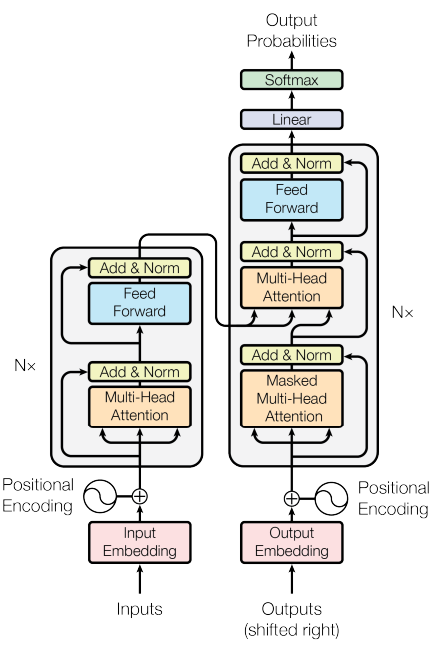
\includegraphics[width=0.6\linewidth]{figures/transformer.png}
    \end{center}
	\caption{Transformer model architecture \cite{Vaswani:2017}. Encoder is on the left; decoder is on the right.}
    \vspace{-5mm}
	\label{fig:transformer}
\end{figure}

\if{false}
\section{Fine-tuning}
\fi